
\chapter{Experimental infrastructure}
	\begin{adjustwidth}{0cm}{0cm}
	\begin{flushright}
	\emph{``Every sensor is a temperature sensor.  Some sensors measure other things too."\\} 
	- Engineer's aphorism\footnote{Quoted without attribution in Elecia White's \emph{Making Embedded Systems}, O'Reilly media, 2011}
	\end{flushright}
	\end{adjustwidth}

	This dissertation spans works conducted on two experimental apparatus. The major works discussed in chapters \ref{chap:spectroscopy} and \ref{chap:QD} were undertaken on an existing machine, which has been in productive operation for many years. This machine achieved BEC in 2007 \cite{dall07}, utilizing a bright cold beam of helium \cite{swansson04} and optimized Zeeman slower \cite{dedman04}. Key technical facilitations were the installation of auxiliary field coils for active cancellation of stray magnetic fields \cite{dedman04} and ambient air temperature control at the centikelvin level at the BEC chamber\footnote{also known affectionately as the \emph{science chamber}.} by control of the cooling air mixture \cite{dedman15}. The machine has had a storied history since then, hosting a range of experimental themes including correlations between many atoms \cite{hodgman17,dall13,manning13} (especially Hanbury Brown-Twiss correlations \cite{manning10,dall11a,hodgman11,rugway11,rugway13}), studies of atom lasers \cite{dall07,dall08a,henson18,manning10} and guided matter waves \cite{dall10, dall11a,dall11}, and quantum-optics demonstrations such as single-particle sources \cite{manning14}, ghost-imaging \cite{khakimov16,hodgman19}, Wheeler's delayed choice thought experiment \cite{manning15}, and bell-type correlations between pairs of freely propagating atoms \cite{shin19}. This machine was also used for proof-of-principle demonstrations of a machine-learning assisted optimization of a quantum transport protocol \cite{henson18ML} and 3D magnetic gradiometry with pairs of atoms \cite{shin20}. While I was a collaborator for each of these two works, they are not included in this thesis. My main work on this machine includes laser spectroscopic studies of helium structure including the 413nm tune-out wavelength (as first reported in \cite{henson15} and improved during the course of this thesis, with publication forthcoming) and transition energies \cite{ross20,thomas20}, and  investigations of the quantum depletion of a condensate as described in chapter \ref{chap:QD}. 
	This machine is described in great detail in past publications (in particular \cite{swansson04,dall07}) and PhD dissertations \cite{hodgmanthesis,manningthesis,shinthesis,dallthesis}. In this section, therefore, the apparatus will be summarily described, and the motivated reader referred to the aforementioned sources for more information, and to the texts \cite{FootAtomic,MetVdS} for general details about cooling and trapping techniques.

	About half the duration of this course of study was devoted to the refurbishment of a retired cold-atom experiment towards loading a \mhe BEC into an optical lattice. Before its erstwhile retirement, this machine was used for the study of electron scattering and  dual-species MOT experiments\cite{uhlmann05,byron10,byron10a}, and determination of electronic transition rates \cite{dall08,hodgman09,hodgman09a} in \mhe \todo{[??] was done downstairs}. The renovation of this machine was motived by the insufficient optical access into the BEC chamber of the already-operating machine, preventing a straightforward upgrade. These machines can be distinguished between these two by their intended final trapping method: The machine discussed in the previous paragraph could therefore labelled the \emph{BiQUIC machine}, and the upgraded apparatus referred to as the \emph{lattice machine}. BEC was recently achieved in the lattice machine by the resident graduate students \cite{abbas21}, and the construction is ongoing. As the lattice machine has yet to produce scientific results in its newfound youth, I will discuss the scientific motivation for its construction and my contributions to the project in chapter \ref{chap:lattice}. This chapter is concerned with the anatomy of the first machine, which hosted the works described in chapters \ref{chap:spectroscopy} and \ref{chap:QD}. The distinctive features of the refurbished machine will be described in chapter \ref{chap:lattice}.

\section{Helium beamline}
	In brief, both BEC machines exist to achieve magnetic trapping of metastable helium in ultra-high vacuum (UHV) conditions \footnote{Sometimes called \emph{hard} vacuum. Both terms are amusingly paradoxical.}. Magnetic trapping is required because the limits of optical cooling are too hot to achieve degeneracy with the conventional densities. Optical cooling techniques are required to achieve low enough temperatures such that the magnetic trap can be filled with a suitable population to reach BEC by evaporative cooling. The pecularities of producing \mhe atoms and the need for multiple optical interfaces into UHV conditions demand large devices with many hundreds of moving parts. 
	\todo{basic mechanism of laser cooling in brief}
	The fundamental minimum for laser cooling by radiation pressure is the \emph{recoil limit} set by the relation $k_B T = \hbar^2k^2/2m$, where $k$ is the wavevector of the cooling light. This is the energy scale fixed by a single-photon emission, and is about 2 $\mu$K for Helium. While this is too hot to achieve condensation in the traps considered in this thesis (whose critical temperature is about 1 $\mu$K), we generally only use laser cooling down to the \emph{Doppler limit}. The latter is given by $T = \hbar\Gamma/2 k_B\approx 38~\mu$K and corresponds to the minimum velocity difference which can be distinguished by the cooling laser. In practise this is set by the linewidth $\Gamma$ of the cooling transition (1.6MHz for the $2\triplet S_1 -- 2\triplet P_2$ transition) , as the laser linewidth is smaller by about an order of magnitude\cite{shin16}. These limits of optical cooling mean that laser cooling of helium to the ground state of our traps is not possible. Furthermore, helium has a spinless nucleus and thus no hyperfine structure, precluding the polarization-gradient cooling employed in alkali atoms. Fortunately, condensation is achievable in magnetic traps. The pathway from room temperature to degeneracy is outlined in the rest of this section.
	% bergeman93 quantum calculations for one-dimensional laser cooling
	% castin89 limits of laser cooling in 1D
	% castin91 theory of sisyphus cooling(polz gradient?)
	% cooper94 temperature of atoms in a MOT
	% doery94 using 1083nm transition to look at lattice effects in optical molasses

% Could possibly calculate total efficiency (He input -> BEC flux (even detection), coefficient of performance as refrigerator, etc)
% There are two experiments described in this thesis. The majority of work is done on the old machine, whose construction is discussed here. At the end of this section, differences with the upstairs machine are noted, and further discussion of that specific machine is left to chapter X.
% The entire device is built in a controlled climate yadda yadda

	% \begin{table}
	% \centering
	% \begin{tabular}{|c | S S | S S|}
	% \hline
	% Beamline stages & \multicolumn{2}{c|}{Detuning} 		& \multicolumn{2}{c|}{Intensity}\\
	% 				& 	MHz & $\Gamma$ 					& mW/cm$^{2}$ 		& $I_\textrm{sat}$ \\
	% \hline
	% Zeeman slower	& -66.6 	& -6.9 						& 133.7 				& 42.0\\
	% MOT 2			& -6.6 	& -69.0 						& 13.37 				& 420.0\\
	% \hline
	% \end{tabular}
	% \caption{Parameters of the cooling and trapping beams in the main machine}
	% \label{aomtable}
	% \end{table}

\subsection*{\mhe atom source}

	The metastable \mhe state is generally produced by a DC electric discharge as opposed to optical excitation due to the lack of convenient X-ray light sources at 63nm. Electons accelerated by a strong potential gradient can ionize helium atoms, and thus also have enough energy to excite atoms into the \mhe state. In our experiments, a grounded copper block cooled by liquid nitrogen serves as the anode and reaction vessel. A tungsten cathode is held at 2kV and placed in front of the vessel, separated by electrically insulating boron nitride spacers. The breakdown voltage of helium gas in this geometry is minimized at a pressure above the standard operating setting, and even then an additional 2.5kV is required to achieve ignition before turning the source pressure down into the operating regime. Unfortunately, the DC discharge only excites about .01\% of the atoms into the \mhe state \cite{stas06}, and multiple collisions impart fairly high velocities to the light helium atoms, despite being cooled by liquid nitrogen. This necessitates a larger Zeeman slower stage than is found in other cold-atom apparatus. \todo{Not necessarily true - there are plenty of zeeman slowers for other atomic species longer than the downstairs zeeman slower.  Even so, most of that is to do with the light mass of He - most atoms requiring a zeeman slower come out of an oven, which may be at temperatures of the high hundreds of degrees, which is far hotter than what comes out of our source (essentially LN2 temperature)}

	The source chamber tends to operate consistently over a year or so, permitting development and execution of a handful of experimental campaigns. However, the copper housing can degrade with time, causing intermittent source extinctions or even preventing successful striking altogether. This can be remedied by extracting the source chamber from the vacuum system and skimming a few microns of copper from the interior surface of the block. This procesure is generally straightforward but somewhat painstaking. 

\subsection*{Beam forming}

	The gas expands out of the forward-facing aperture of the reaction vessel and a small solid angle is selected by a skimming nozzle between the source chamber and the rest of the helium beamline. The skimmer serves a secondary purpose as a weak differential pumping stage \todo{it's whole purpose is kind of for differential pumping - the small solid angle is to select atoms with low transverse velocity while rejecting (i.e. differentially pumping) everything else.}, keeping the first laser cooling stages at a lower pressure than the source chamber. The beam is collimated\footnote{Technically speaking, the beam is not collimated in the same manner as a laser beam. The divergence is reduced, but not enough for the beam to converge to a focus further along the beamline. Similarly, the `focus' stage described below does not create a convergence but provides additional transverse cooling.} by a single beam reflected in a figure-4 configuration\todo{this is not standard... rephrase or ?}, forming a a 2D optical molasses\cite{Lett81,rooijakkers96} and providing cooling in the two transverse degrees of freedom. This is followed by a `bending' stage wherein a single beam, picked off from the collimator, deflects the metastable atoms by a few degrees through a second stage of differential pumping into the Zeeman slower chamber. This provides better selectivity of \mhe atoms by reducing the number of unexcited atoms that enter the Zeeman slower and first MOT chambers. \todo{by blocking line of sight to the MOT}
	% \subsection*{Optical molasses}
	% P D Lett, W D Phillips, S L Rolston, CE Tanner, R N Watts, C I Wetbrook, Optical Molasses, journal of the optical society of america B 6, 2084-2107, Nov 1981
	% W Rooijakkers, Wo Hogervorst, W Vassen, an intense collimated beam of metastable helium atoms by two-dimensional laser cooling, Optics COmmunications 123, january 1996

	Zeeman slowers, so named for the exploitation of the Zeeman effect \todo{be more specific, as the Zeeman effect is used all over the place}, are necessary to slow atoms from thermal velocities imparted from their sources to below the capture velocity of the magneto-optical traps located at the end of the slower. The Zeeman slower in our experiment \cite{dedman04}  reduces the most probable longitudinal velocity of the beam from $\approx700$ m/s to $\approx70$ m/s, which permits loading of the MOT to a steady-state population in about one second.

	% W Rooijakkers, Wo Hogervorst, W Vassen, an intense collimated beam of metastable helium atoms by two-dimensional laser cooling, Optics COmmunications 123, january 1996

\subsection*{First Magneto-Optical Trap}

	The magneto-optical trap combines the radiation pressure with a spatially-varying magnetic field. When atoms move away from the centre of the trap, a restoring force is created as the atoms move into resonance with one of the six counterpropagating laser beams along the $x,~y,$ or $z$ axis. A quadrupole magnetic field ensures atoms are resonan\todo{It doesn't really ensure they are resonant, because you have to consider their velocity too, more that it increases the scattering probability by creating a spatially varying restoring force. (I'm sure you could explain that in a better wording)} as they approach an ellipsoid surrounding the trap centre, thus confining atoms within the trapping area. This technique was first proposed by Jean Dalibard and eventually realised by Raab \emph{et al} \cite{raab87}. Early helium MOTs were limited in number because of the size of the trap. Later attempts achieved larger number by operating with larger beams and detunings (-22$\Gamma$), obtaining lower densities than in other species \cite{tol99} and mitigating losses due to Penning ionization. The multifaceted physics of MOTs has proven rich ground for study in general \cite{Townsend95,walker90}, and also in the specific case of helium, for which the two-body loss rate has been studied \cite{tol99} along with the roles of light-assisted collisions \cite{papers}. Temperatures in a MOT are, at best, on the order of the steady-state molasses temperature $\approx1$ mK \cite{Lett81}. Further evaporative cooling is therefore required to reach quantum degeneracy.
	% P J J Tol, N Herschbach, E A Hessels, W Hogervorst, W Vassen, alrge numbers of cold metastable helium atoms in a magneto0optical trap, physical review A 60, august 1999
	% E L Raab, M Prentiss, A Cable, S Chu, D E Pritchard, Trapping of neutral sodium atoms with radiation pressure, Physical Review Letters 59, 2631-2634, Dec 1987
	% P D Lett, W D Phillips, S L Rolston, CE Tanner, R N Watts, C I Wetbrook, Optical Molasses, journal of the optical society of america B 6, 2084-2107, Nov 1981
	% C G Townsend, N H edwards, C J cooper, K P zetie, C J foot, A M Steane, P Szrfitgiser, H Perrin, J Dalibard, Phase-space density in the magneto-optical trap, Physical review A 52, august 1995
	% T Walker, D sesko, C E Wiemann, collective behaviour of opticlly trapped neutral atoms, physical review letters 64, jan 1990
	The background pressure in the first MOT chamber is still too high to maintain a long-lived magnetic trap. Therefore, the first MOT is used as a source for a secondary helium beam which feeds into the final science chamber. The MOT chamber features a $\approx$2mm hole bored through a compound quarter-waveplate-and-mirror mounted inside the vacuum chamber, which adjoins the transfer conduit supplying the BEC chamber with cold helium. \todo{point to schematic}

	A slightly blue-detuned `push' beam is aligned with the aperture at the back of the first MOT to transfer atoms into the second MOT along ballistic trajectories \cite{swansson04}. In practise the beam points slightly upward, and the orientation is optimized by maximizing the saturated fluorescence signal in the second MOT. The atoms pass through a `focus' stage consisting of two crossed, retro-reflected laser beams with a $\approx$1cm waist. Wire coils mounted around the 2$\frac{3}{4}$" window flanges create an octupole \todo{Is it just a pair of coils? I thought there was one on each window...} magnetic field surrounding the beamline such that the circularly-polarized beams address only atoms on the proximal half of the beam to the optical insertion. This provides a final stage of transverse cooling and increases the efficiency of loading the second MOT from the \mhe beam. The focusing stage typically increases the saturated fluorescence signal in the second MOT by at least 50\%. 

\subsection*{The Science Chamber}

	The second trapping chamber is evacuated to a pressure of some $10^{-11}$ mbar, which provides an excellent magnetic trap lifetime of several minutes \todo{remove minutes claim or show some data}. The chamber is surrounded by three pairs of square magnetic coils which actuate active cancellation of stray fields from the earth and nearby electronic equipment\footnote{The `nuller' reduces, but does not eliminate, 50Hz noise from the AC mains supply to the laboratory.} \cite{dedman07}. This assists the creation of a stable magnetic trap with two coil pairs in a Bi-planar quadrupole Ioffe configuration (BiQUIC) \cite{dall07}. Magnetic traps exploit the interaction of the atomic magnetic dipole with a magnetic field, which takes the form $E_B = -\mu\cdot \textbf{B} = -\hbar g m_J B$. A magnetic field with a local extremum can therefore form a confining potential for the states whose energy is minimized at this point. It follows from the Maxwell equations that a magnetic field in free space cannot have any local maxima \cite{MakingProbingUnderstanding}, and so one must select an atomic state with $g m_J>0$ for confinement at a local minimum of the magnetic field. In \mhe this uniquely selects the $m_J=+1$ state for magnetic trapping, which also ensures complete spin-polarization and the attendant reduction in Penning losses. The BiQUIC design is a solution to a critical issue with early traps \cite{migdall85}: The quadrupole fields generated by coils in an anti-Helmholtz configuration feature a zero crossing in the trap centre. Atoms in a magnetic field undergo transitions to untrapped states, known as \emph{Majorana transitions}, at a rate proportional to $\exp(-B/\omega)$, where $\omega$ is the trapping frequency and $B$ is the magnitude of a (uniform) magnetic field \cite{sukumar97}. In harmonic traps the trap bottom thus sets the upper bound on the Majorana transition rate \cite{brink06}. Many variations on the quadrupole trap exist to mitigate this issue, including the Time-Orbiting Potential (TOP) \cite{petrich95}, Ioffe-Pritchard \cite{pritchard83}, cloverleaf \cite{mewes97}, and QUIC \cite{esslinger98} traps. Other groups have added a repulsive dipole potential to the trap zero with a focused and blue-detuned laser beam \cite{papers}. 
	% harms00 Earnshaw's theorem shows that a static potential cannot trap a charged particle, not a statement about neutral particles
	% T. Esslinger, I. Bloch, and T. W. H¨ansch, “Bose-Einstein condensation in a quadrupole-Ioffe-configuration trap,” Phys. Rev. A 58, R2664–R2667 (1998).
	% M.-O. Mewes, M. R. Andrews, N. J. van Druten, D. M. Kurn, D. S. Durfee, and W. Ketterle, “Bose-Einstein Condensation in a Tightly Confining DC Magnetic Trap,” Phys. Rev. Lett. 77, 416–419 (1996).
	% 	D. E. Pritchard, “Cooling Neutral Atoms in a Magnetic Trap for Precision Spectroscopy,” Phys. Rev. Lett. 51, 1336–1339 (1983).

	% D. G. Fried, T. C. Killian, L.Willmann, D. Landhuis, S. C. Moss, D. Kleppner, and T. J. Greytak, “Bose-Einstein Condensation of Atomic Hydrogen,” Phys. Rev. Lett. 81, 3811–3814 (1998).
	% J. Fort´agh and C. Zimmermann, “Magnetic microtraps for ultracold atoms,” Rev. Mod. Phys. 79, 235–289 (2007).

	In addition, a pair of low-intensity Doppler cooling beams \todo{insert doppler cooling explanation, probably in earlier section. } are inserted at 15$^\circ$ relative to the horizontal. A vacuum window on the opposite side to the helium beam provides optical access for a spectroscopic probe beam or the 1550nm beams used for atom-optics techniques (employed in works not relevant to this thesis). The final optical component is a diagnostic photodiode mounted outside the chamber and is used to measure a saturated fluorescence signal\todo{define what this is}, which serves as a diagnostic for the in-trap population. Two radio antennas provide the RF signals for the evaporative cooling and atom lasers, respectively. The evaporative cooling ramp is generated by an arbitrary waveform generator pre-loaded with a time-varying frequency ramp created with the LabView control software (see below). The secondary coil is driven by a function generator, and both signals are passed through separate dedicated 30W amplifiers before insertion into the chamber.



\section{Light sources}\label{ssec:lasers}
	
	The principal light source for both experimental apparatus is the 1083nm cooling and trapping laser. The light source is an external-cavity diode laser which is depicted in Figure \ref{fig:main_laser}, published in \cite{shin16} and detailed in the PhD thesis of D. K. Shin \cite{ShinThesis}. The laser output passes through an in-fibre beamsplitter, of which one output is blue-shifted by 253MHz by an acousto-optical modulator (AOM) and locked to a helium gas cell by saturation absorption spectroscopy. The remaining arm is coupled by optical fibres to the fibre amplifiers of both experiments. The supply of light which is 253MHz red of the field-free resonance reduces the risk of stray light interacting with atoms and disrupting the delicate cooling and trapping processes \todo{Also, if it was close to resonance then you couldn't use AOMs to generate all the different frequencies we need for the many cooling and trapping beams}. Each experiment features its own fibre amplifier that produces up to 5 W of laser power from the $\approx$3 mW supplied by the ECDL. The lattice machine also makes use of 1550nm light, whose generation and application is discussed in chapter \ref{chap:lattice}.
	% N Herschbach, Trrapped Triplet helium atoms: inelastic collisions and evaporative cooling, PhD thesis VU Amsterdam 2003

	\begin{figure}
		\centering
		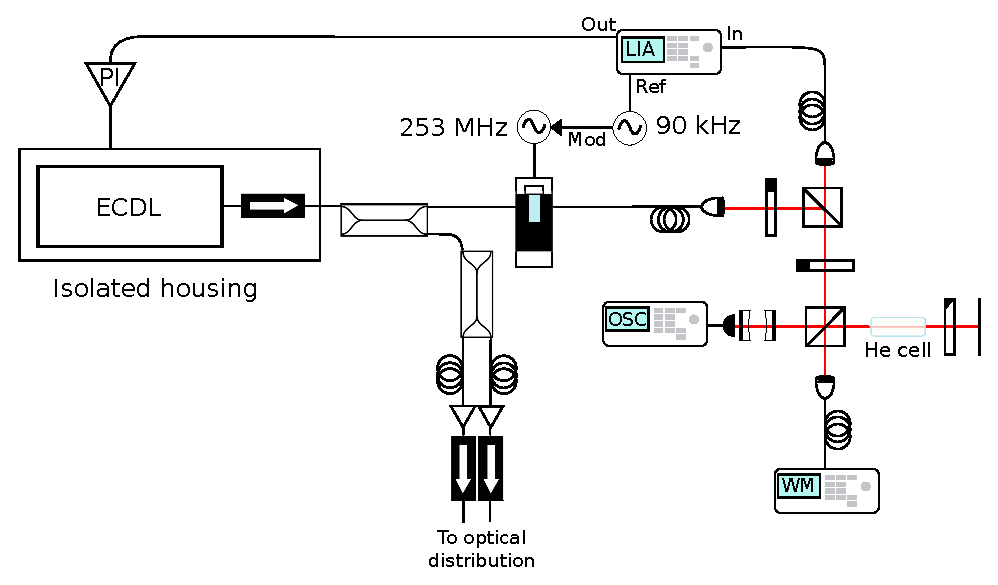
\includegraphics[width=\textwidth]{fig/apparatus/master_laser_system}
		\caption{Schematic of the generation and control system for the main cooling laser operating at 1083.331nm. \todo{double check unused channel} \todo{Put this later/after the main exp schematic}}
		\label{fig:main_laser}
	\end{figure}
	
	
	% Both machines also employ sources of 1550nm laser light, used for a crossed optical dipole trap in the lattice machine, and to implement atom-optical control elements in the BiQUIC machine. The latter techniques are mentioned here for completeness but are not discussed further as they were not used in the works in this thesis. The construction and operation of the 1550nm optics for the lattice machine are described in chapter \ref{chap:lattice}.

	% http://www.heliumbec.com/wiki/February_2017_Bake
	% https://imgur.com/a/4BxKh
	% http://www.heliumbec.com/wiki/Titanium_Sublimation


\subsection*{Optical distribution setups}

	\begin{figure}
		\centering
		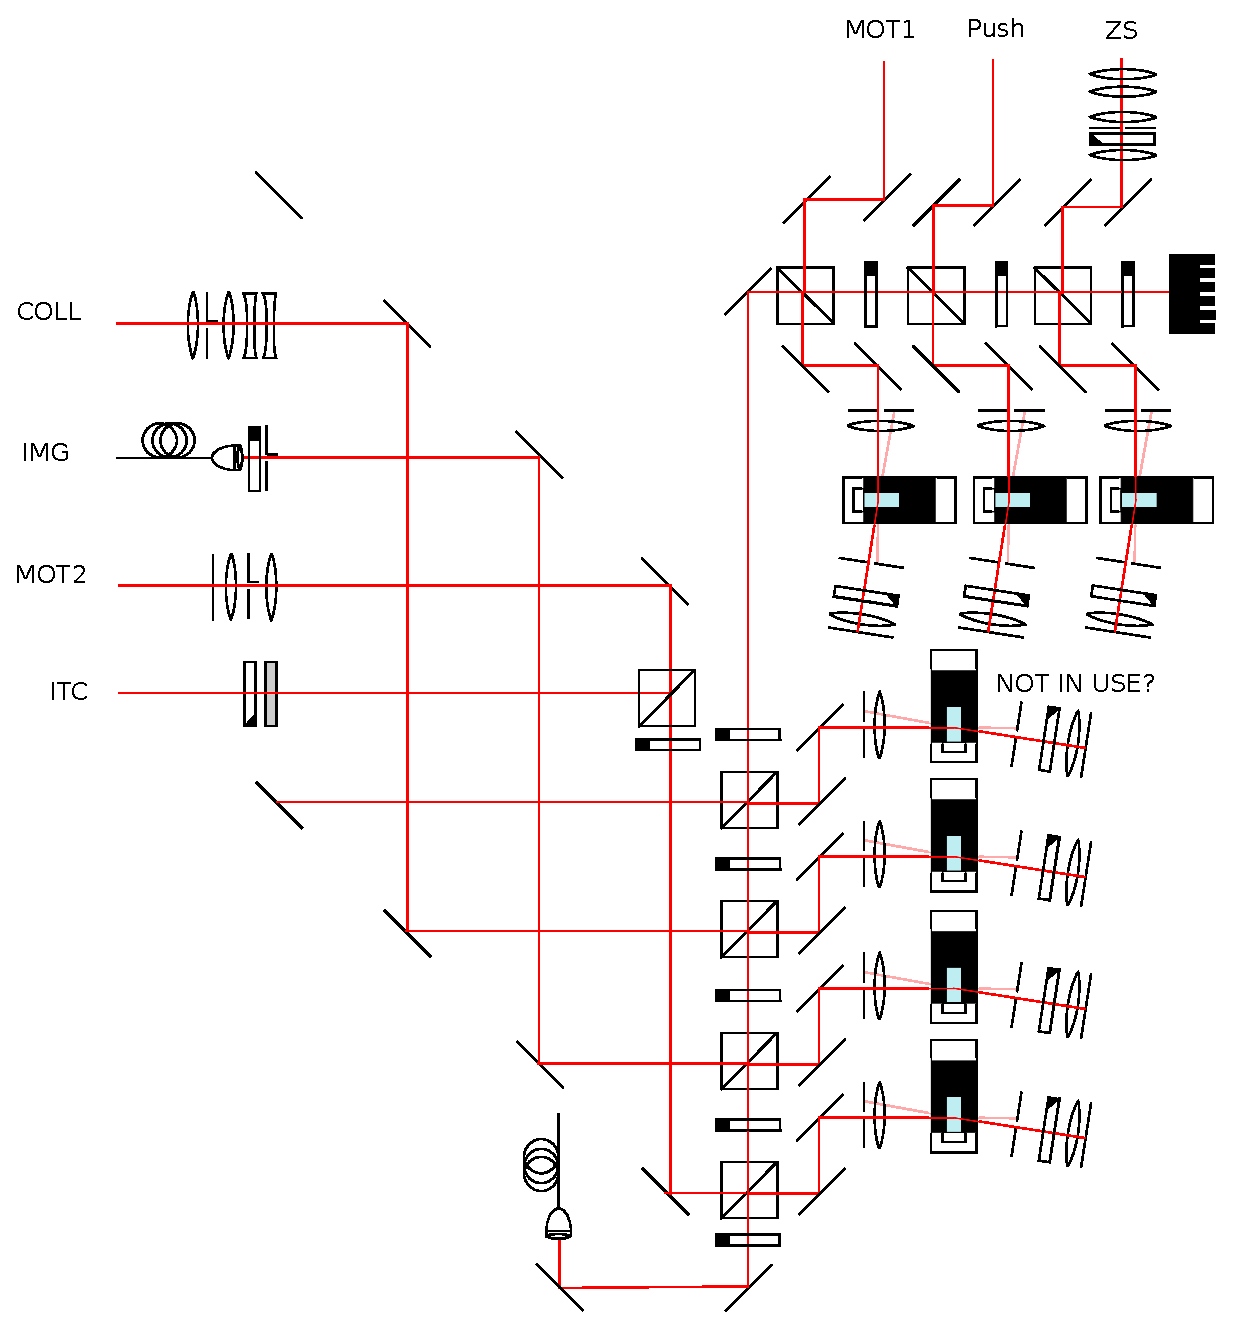
\includegraphics[width=\textwidth]{fig/apparatus/lattice_cooling_optics}
		\caption{Schematic of the control and distribution system for cooling light in the lattice machine. \todo{This schematic is hard to follow, as it's hard to see what beam path is which.  Also, I'm not sure what information it conveys, given that each beam is essentially a copy of the others (in terms of the functional information this diagram shows).  You'd need to label things like AOMs, waveplates etc and probably highlight each beam in different colours or somehting for it to be useful, but I'd probably just not include it. }}
		\label{fig:lattice_cooling_optics}
	\end{figure}
	
	In each machine, a suite of AOMs are used to independently control the power and frequency of each of several specialized beams \footnote{The active component of an AOM is a crystal is driven at radio frequencies by an amplified voltage-controlled oscillator. An acoustic standing wave, constituted by phonons with frequency matched to the driving frequency, scatters light into discrete diffraction modes width momenta shifted by the phonon-lattice momentum. The action is analogoous to a diffraction grating, and described by the Kapitza-Dirac mechanism. Thus the AOM transduces electronic signals into optical frequency shifts. An analogous effect, with the role of atoms and light interchanged, is the operating principle of optical lattices.}. The first-order diffraction is usually chosen for its more efficient transmission. The pointing of the diffracted beams vary with the AOM frequency, which is a problem when the ultimate destination of the light is separated from the AOM by several meters of optical path length, after which the deflection can become significant. To circumvent this, the AOMs are set up in a double-pass `cat's-eye' configuration so the deflection in one pass is canceled by the second pass in the opposite direction.
	
	The AOM suites are supplied by light picked off from the output of the fibre amplifier by a half-waveplate and beamsplitter pair per AOM, as depicted in \ref{fig:lattice_cooling_optics}\footnote{This figure shows the AOM suite layout for the lattice machine, as I built it when working on the project. The layout for the BiQUIC machine is essentially the same.}. A quarter-wave plate placed in the optical path through the cat's-eye ensures the doubly-diffracted beams are transmitted back through the beamsplitter into the distribution optics. AOMs offer the advantage of fast switching times, but some light can leak from the AOM suite through the optical paths into the experiment. As such we used electronic shutters and an opaque enclosure to prevent this from occurring. The shutter action as well as the detuning and diffraction efficiency of the AOMs are actuated by the control software described later in this chapter. 
	


\subsection*{Spectroscopic laser}
	A light source unique to the BiQUIC machine was the tunable laser system used to generate light in the $402-430$nm range for the laser spectroscopy measurements discussed  in Chapter \ref{chap:spectroscopy}. This  was a tunable M-squared Ti:Sapphire laser system, depicted in Figure \ref{fig:tunable_laser}. Light at 1064nm from a Lighthouse Photonics Sprout module was frequency doubled by second-harmonic generation to pump an M-squared SolsTi:S titanium-sapphire laser which we operated around 800nm. The output from the SolsTi:S was doubled again in an M-squared ECD-X module to the target wavelengths. A fraction of the light is fed into a High Finesse WS-8 wavemeter. High Finesse specifies the absolute accuracy of the WS-8 at 2MHz within 2nm of a transition line, and 10MHz otherwise. We use the wavemeter to lock the tunable laser with respect to the red light, so the uncertainty is doubled in determinations of the blue frequency. We calibrated the wavemeter once every day or so with respect to the two-photon crossover transition between the $6^2P_{\frac{3}{2}} (F=4)$ and $6^2P_{\frac{3}{2}} (F=5)$ lines in a cesium vapor cell. We used saturated absorption spectroscopy to lock the red light to the Cs transition while feeding light into the wavemeter for the calibration.	A MATLAB software lock uses the wavemeter output to stabilize the laser to within 100kHz of the target wavelength, and allows automatic scans across the region of interest by automatically updating the laser set point. \todo{description of TCP lock protocol}

	\begin{figure}
		\centering
		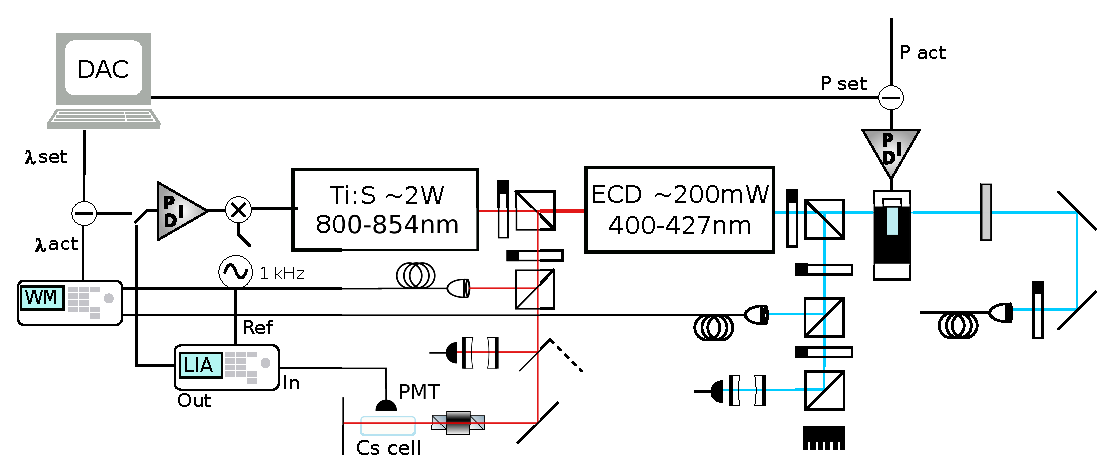
\includegraphics[width=\textwidth]{fig/apparatus/solstis_schematic_minim}
		\caption{Schematic of the spectroscopic laser system, including calibration infrastructure. \todo{Probably need  a bit more detail in teh caption, especially as it doesn't all seem to be in teh main text.}}
		\label{fig:tunable_laser}
	\end{figure}
	
	

	We used the first diffracted mode of an AOM, driven at 189MHz, to control the beam power. The output of the AOM was fed into an optical fibre which coupled the light to the vacuum insertion optics. There, we used waveplates to set the polarization and a telescope to magnify the beam up to $\approx$2cm waist. A final lens fixed to a three-axis translation mount was used to focus and align the beam. For the measurements of the tune-out and forbidden transition wavelengths, we focused the beam to a diffraction-limited waist, about $100~\mu$m at the site of the BEC, to achieve strong interaction given the weak signals of interest \todo{double check that waist size. I think it was actually smaller, on the order of the TF radius}. For the $2\triplet P_2\rightarrow 5\triplet D$ transitions described in the bulk of Chapter \ref{chap:spectroscopy}, the beam was collimated and operated at a reduced power to mitigate power broadening and saturation of these much stronger resonances. The optical power was regulated with reference to a photodiode which sampled the beam after the fibre via a polarizing beamsplitter.

	The wavemeter logs, photodiode voltage, and transmission of light from both the 800nm and 400nm beams through two scanning Fabry-Perot cavities (SFPs) were recorded through the DAC system in order to provide diagnostics in post-processing. Part of the data analysis pipeline then automatically discarded shots where either SFP showed multiple peaks within a single free-spectral range (FSR), indicating that one of the lasers was running in am ultimode regime, or where the photodiode trace indicated a laser supply failure, or where other anomalous behavioru was detected.


	% Camera/mirror setup Reproducibility
	% issues

\section{Detection of metastable helium atoms}

	A unique diagnostic available in helium experiments is the production of helium ion-electron pairs. This process can be monitored by in-vacuum electron multipliers mounted near the trapping region. Proximity to the trap is desirable for efficient collection of the resulting particles. Aside from investigating Penning ionization itself (as mentioned earlier in this chapter), ion detection has been applied in photoassociation spectroscopy \cite{herschbach00,koelemeij04}, to monitor the onset of Bose-Einstein condensation \cite{tychkov06}, and for high-precision laser spectroscopy \cite{Rengelink18}. The ion detector in the BiQUIC machine stopped working some years ago and has not been replaced: the utility of this diagnostic is outweighed by the effort required to break vacuum for the first time in a decade or so, disassemble the chamber and surrounding optics, reassemble everything, bake the chamber, and realign all the optics. As such ion detection garners only a brief mention in section \ref{sec:DipoleAlignment}, wherein I describe an attempt to use the ion detection as an diagnostic to aid alignment of a dipole beam in the lattice machine. In an accident a year or so after I left that lab, the ceramic feed-throughs connecting the ion detector to the external electronics cracked. This broke vacuum, necessitating a rebake of the chamber, and saw the detector retired. 

	Two optical detection methods are employed in the ANU helium labs. Saturated fluorescence measurements are used to monitor the number of atoms in a trap. In this method, bright resonant light ($I\gg I_\textrm{sat}$) is applied to the atoms such that the population of the excited state saturates at 50\%. If the light is applied while the trap remains on, then while some atoms may decay to a trapped state, repeated absorption events eventually drive them out of the trap. Therefore, one expects a sharp peak and subsequent decay in the optical power re-emitted from the trap. This radiation can be captured by a lens and focused onto a photodiode, producing an analog voltage as a useful diagnostic. The difference between peak and steady-state voltage after the pulse is a direct probe of the atomic population. This technique is generally employed only as a diagnostic tool for fast readout when optimizing the alignment of cooling and trapping beams, and as such will not be discussed in further detail. The second optical interrogation technique, resonant absorprtion imaging, is only available in the upstairs laboratory. Therefore the theory, construction, and use of the absorption imaging apparatus is discussed in Chapter \ref{chap:lattice}. \todo{Maybe put maintenance after this as it's defined the sat fluro, which is better than just a diagnostic, you can make accurate number measurements with it}


\subsection*{Single-atom detection with the MCP-DLD stack}
% http://www.heliumbec.com/wiki/Detectors
	The principal detection scheme in this thesis is single-atom sensing in the far-field regime using a multichannel plate and delay-line detector combination (MCP-DLD). In some experiments, such as those conducted by the \mhe group at VU Amsterdam, the MCP itself can be used as an ion- or metastable-atom detector. In our experiments, the MCP is paired with either a phosphor screen (usually only used for diagnostic purposes) or with a delay line detector to form the MCP-DLD, which is the workhorse of most experiments conducted at ANU. A summary description is given here, and detailed explanations of the detector stack and signal processing pipeline can be found in \cite{ShinThesis, HodgmanThesis, ManningThesis}. The MCP consists of two plates, each of which feature 10$\micron$-diameter pores arranged in a square grid with 20$\micron$ between the centres of the pore openings . The plates are 80mm in diameter, with the upper surface 848mm below the BiQUIC trap centre. The freefall time-of-flight of the centre of mass of the cloud is 417ms, which means the maximum measurable horizontal velocity is about 9.5 m/s, sufficient to capture almost all of the thermal fraction for clouds below the critical temperature. The detector plates are grounded for most of the experimental sequence, and then the top plate is ramped to -2.4kV over about 2 seconds before dropping the trap. The negative voltage repels electrons from the surface of the plate which protects the detector surface from degradation and reduces the background count rate. The background rate, also called the \emph{dark count} rate, is 0.56 Hz/cm$^2$ when operating at -2.4kV, which is practically negligible for the purposes of experiments in this thesis \todo{Maybe include a figure showing this dark rate?}. 

	\todo{MCP-DLD schematic}
	When an atom strikes the surface of a pore after falling from the trap, a second-order process releases an electron with most of the  19.8eV as kinetic energy\cite{ThatPaper}. These electrons are accelerated down the pore by the strong electric field, and themselves impact the pore surface and eject more electrons, triggering an electron avalanche that amplifies each atom impact into over 10$^6$ electrons. The electron shower exits the back of the detector and is accelerated by a +300V potential towards the delay-line detector (DLD). The DLD in the BiQUIC machine consists of two coils of wire each wound in a helical pattern and arranged perpendicular to one another.  The arrival of an electron cascade causes a current pulse to travel along each wire in both directions from the point of impact. The pulses pass through a fast pre-amplifier and then through a constant-fraction discriminator which converts the analog pulses into a digital signal. Both these processes take place within a Roentdek DLATR6 which is located outside the vacuum chamber. The digital pulses are transmitted to a Roentdek TDC8HP time-digital converter (TDC) which registers the arrival time, relative to the arrival of the main trigger signal from the LabView control software, and writes these to a \verb|*d.txt| file as \verb|(channel,time)| pairs. Finally, a custom C++ script passes over the file and converts the timing data to \verb|(t,x,y)| tuples. The conversion from \verb|(channel,time)| to \verb|(t,x,y)| is performed separately, and indeed the latter usually by a different machine, so as to provide maximum CPU availability to the acquisition function.	Further details about the architecture, construction, and calibration of these detectors is found in \cite{HodgmanThesis,ManningThesis}.

	A second MCP, backed by a phosphor screen and a mirror at 45$^\circ$ to the vertical axis, is mounted on an in-vacuum translation stage below the main chamber. The mirror directs light from the phosphor screen to a CCD camera mounted outside the vacuum chamber. This detection method is not typically used for scientific purposes, but is a useful additional diagnostic when the MCP-DLD detector stack appears to be faulty. The phosphor screen does have a much larger dynamic range than the DLD, however, which makes it useful for visual spotting of subtle distortions in the BEC profile, such as used in the alignment of the spectroscopic probe beam, as described in chapter \ref{chap:spectroscopy}. 


	% % NTM [185] derivation of detector flux profiles - inc mean field 
	% % % Tychkov PhD thesis
	% % RGL [98] calibration of QE - depends on plate voltage, which in turn affects plate lifetime and rate of degradation of QE 
	% % % van Rooij PhD thesis
	% % RGL MCP flux models [94] inc BEC flux in terms of chemical potential 
	% % % van Rooij PhD thesis
	% % TKV [9,10] expanding condensate density distributions 
	% % % Y Castin, R Dum, bose-einstein condensation in time-dependent traps, Physical Review Letters 77, 1996
	% % % F Dalfovo, S Georgini, L P Pitaevskii, S stringari, theory of bose-einstein condensation in trapped gases, rev mod phys 71, april 1999
	% % SSH [38,39] condensate ballstic expansion 
	% % % Castin & Dum
	% % % K. Dieckmann, Bose-Einstein Condensation with High Atom Number in a Deep Magnetic Trap, Ph.D. thesis, University of Amsterdam (2001).
\subsection*{Atom lasers}


	% 	NB - the Einstein coefficients have a cubic dependence on frequency (See also the natural lifetime) and so optical transitions tend to exhibit spontaneous decay more quickly than the Rabi oscillations, but radio transitions (as in the fine structure states) fall much more slowly and coherent oscillations can be seen 
	% One can see that at large detunings, the oscillation frequency ncreases but the amplitude falls off like the detuning-squared, and one instead encounters the dipole potential, right?

	The most straightforward way to use an MCP-DLD to interrogate a BEC is simply to drop the atoms onto the detector. An example of this straightforward detection scheme is illustrated in Fig. \ref{fig:dropped_bec}. A drawback of this method is that the high atom fluxes in large BECs can temporarily deplete the available current carriers near the surface of the detector, resulting in a nonlinear reduction in detection efficiency known as \emph{saturation}. This means that for even moderately sized condensates, a determination of the condensate population by counting detection events or by straightforward fitting of the time-of-flight profile is impractical, and one cannot compute interesting quantities like correlation functions with meaningful accuracy. Another limitation of the trap-release method is that it is a completely destructive measurement - one cannot re-trap the cloud or only drop part of it, which slows down data acquisition for even simple purposes like determining the trapping frequencies. Atom laser methods can circumvent both of these issues. 
	\todo{Put figure closer, but keep on opposing pages}

	The basic principle of an atom laser is to transfer some portion of the condensed atoms into a state that is no longer confined by the trapping potential. This was first achieved by applying pulses of RF radiation to a magnetically trapped condensate shortly after the first realisation of BEC\cite{mewes97}. Later, a continuous-wave atom laser was demonstrated and used to perform RF spectroscopy of the cloud, revealing the symmetry-breaking action of gravity which pulls the BEC away from the minimum of the magnetic field \cite{bloch99}. Optical Raman transitions\footnote{In atom optics, \emph{Bragg} transitions, which impart a momentum transfer, are distinguished from  \emph{Raman} transitions which also induce a change in the electronic state.} can also be used as the outcoupling mechanism \cite{Hagley99} with the advantage of imparting a controllable momentum to the outcoupled atoms, but are not employed in the works in this thesis. 

	Atom lasers are so named because the trapped condensate acts as a reservoir of coherent matter waves, in analogy to lasers as a source of coherent light \cite{narashewski,glauberXX}. The first-order coherence of atom lasers is evident from the observation of interference fringes between matter-wave beams \cite{andrews97} and the higher-order coherence manifests in the many-particle correlations detected in \mhe atom lasers \cite{SomeMorePapers}. Atom lasers can also be collimated \cite{bloch99}, directed with collimated laser beams playing the analogous role of an optical waveguide \cite{Guerin06,couvert08}, and manipulated with optically-induced `mirrors' and beamsplitters \cite{Bloch01}. The potentially continuous operation of atom lasers \cite{Chikkatur02} brings the analogy with conventional lasers even closer. Atom laser physics has been studied in detail and widely deployed through the field of atom optics in the two intervening decades since their conception, including most of the works described in this thesis.
	
	% NB this Andrews paper makes some interesting points about the nature of the condensate order parameter, arrguments about whether BEC is actually coherent/hhas a phase, and the relationship between gauge symmetry breaking and particle number conservation - c.f. that recent paper about number fluctuations in a condensate, discuss in overview


	A simple explanation of the mechanism of an atom laser requires a two-level atom with magnetically trapped and untrapped states labeled $\ket{1}$ and $\ket{0}$. An RF pulse tuned to the splitting $\omega_{10}$ for a duration $t$  induces an oscillation between the two states with Rabi frequency $\Omega$. For an ensemble of $N$ atoms, the independent single-particle oscillations produce a many-body product state which evolves as \cite{mewes97}
	\begin{equation}
		(\cos(\Omega t/2)\ket{0} + \sin(\Omega t/2)\ket{1})^{\otimes N} = \sum_{n=0}^{ N}\sqrt{\frac{N!}{n!(N-n)!}}\cos(\Omega t/2)^{N-n}\sin(\Omega t/2)^n\ket{N-n,n},
	\end{equation}
	where $\ket{N-n,n}$ denotes the state with $n$ atoms coupled out of the trapped state and $N-n$ atoms remaining. The outcoupled fraction is then $\sin^2(\Omega t/2)$.
	 % Examples of the dependence of outcoupled rate with frequency can be seen in figure X. \footnote{There is the question of when the atoms actually leave the trap. In one picture, the RF pulse simply allows the atomic wavefunction to couple periodically to the decay channel corresponding to collision with the detector. So they don't actually 'leave' the trap until there's a detection event. How does one ensure we have no significant coupling to the -1 state, which would miss the detector?}

	In practise, the Zeeman splitting varies across the trap due to the inhomogeneous magnetic field, and so a narrow RF pulse would only be resonant with a section of the condensate. While offering detailed spectroscopy of the condensate, this can be circumvented by applying short RF pulses resonant with the minimum Zeeman splitting of the trap. If such pulses are sufficiently short, the Fourier broadening of the finite-duration pulse is wider than the RF width of the condensate. The typical radio-frequency width of the condensate, i.e. the difference between the resonant frequency at the centre and the edge of the condensate, is set by the chemical potential of the condensate and is typically less than 10kHz in our experiments. An example of the MCP-DLD readout from a pulsed atom laser is shown in Figure \ref{fig:pal_micro}. \todo{So what parameters do we use for our atom lasers then?  All this background is fine, but in a chapter on the experiment you need some more details of what our system actually has}
	% Therefore, an RF pulse duration of order X sec is sufficient to ensure a uniform transfer across the trap. This broadening also dominates the additional shift in Zeeman splitting by the mean-field interaction, which is of order Y kHz. 
	 % The pulses typically on the order of 100$\mu$s long, which for a typical trap splitting of order 2MHz ensures the spectrum of the pulse has a FWHM of order xMHz thanks to Fourier broadenin. 

	 \newpage
	 \begin{figure}
	 	\centering
	 	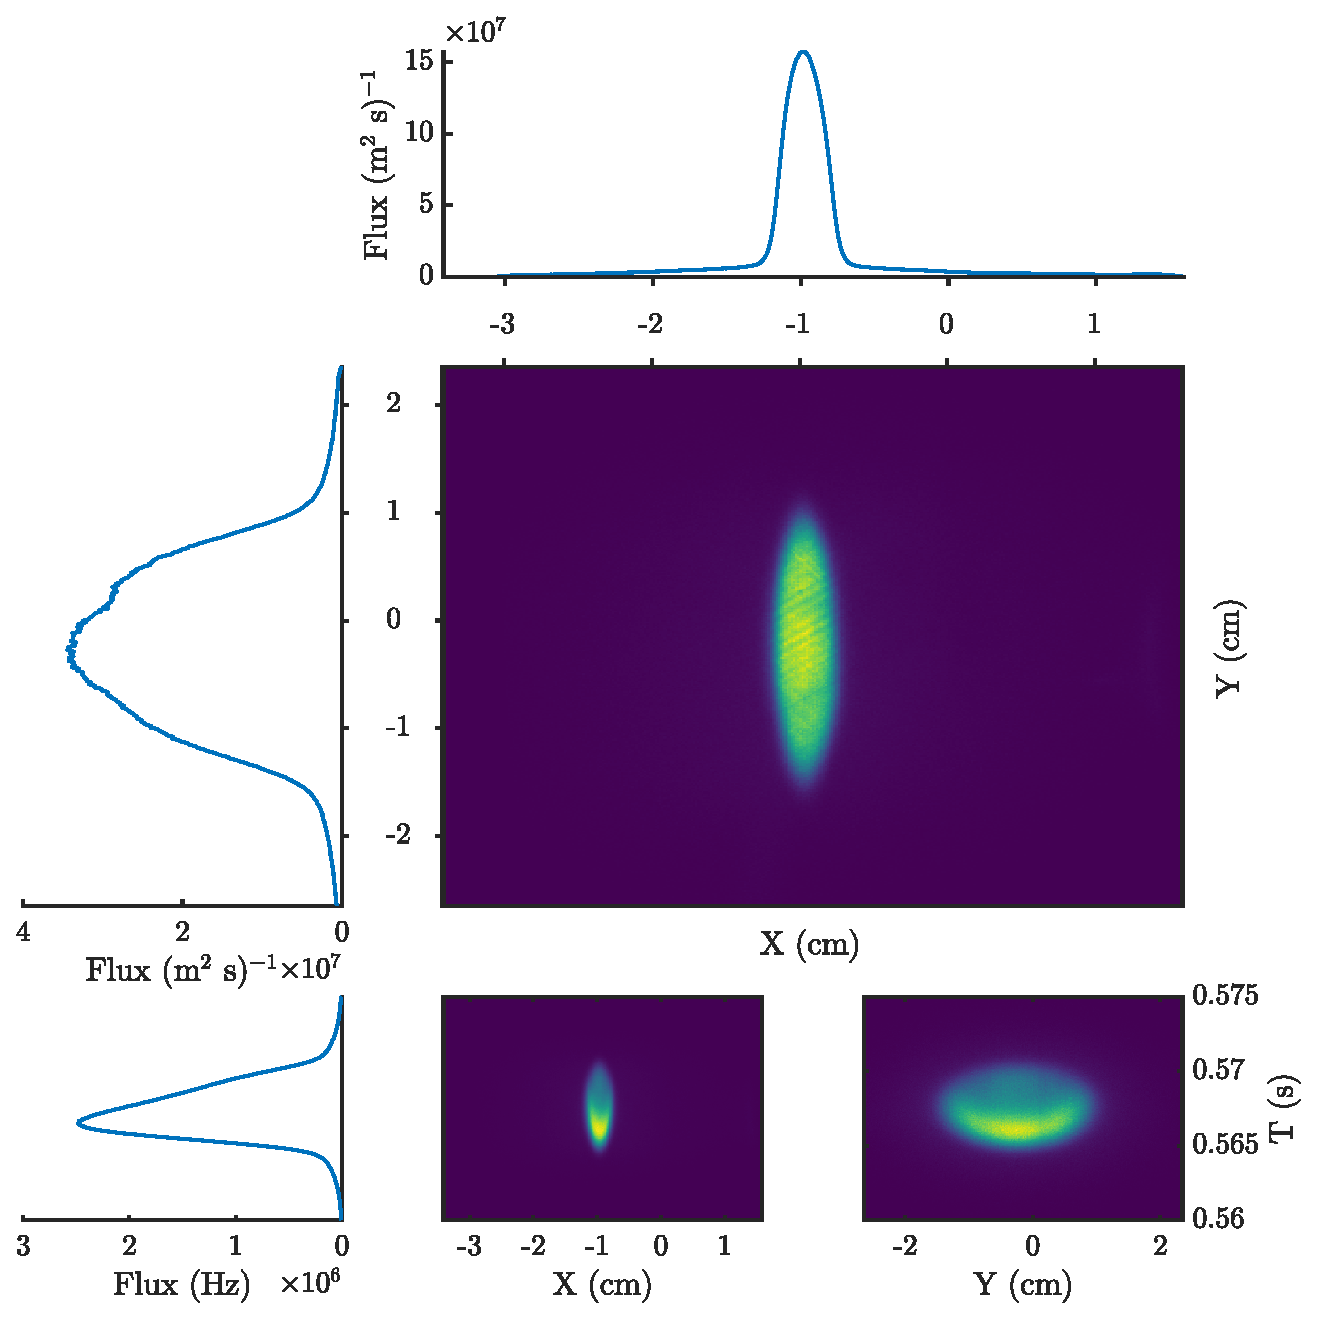
\includegraphics[width=\textwidth]{fig/apparatus/dropped_bec}
	 	\caption{MCP readout of a dropped BEC with small thermal fraction. The detector saturation is evident in the time-of-flight profiles (bottom row) as a sudden downturn in the detected flux, whereas the full BEC has a parabolic profile. The density- and space-dependence of the saturation is visible in the 2D sections (lower middle and lower right).\todo{More axis labels and ticks and such... But they're all common...}}
	 	\label{fig:dropped_bec}
	 \end{figure}

	 \newpage
	 \begin{figure}
	 	\centering
	 	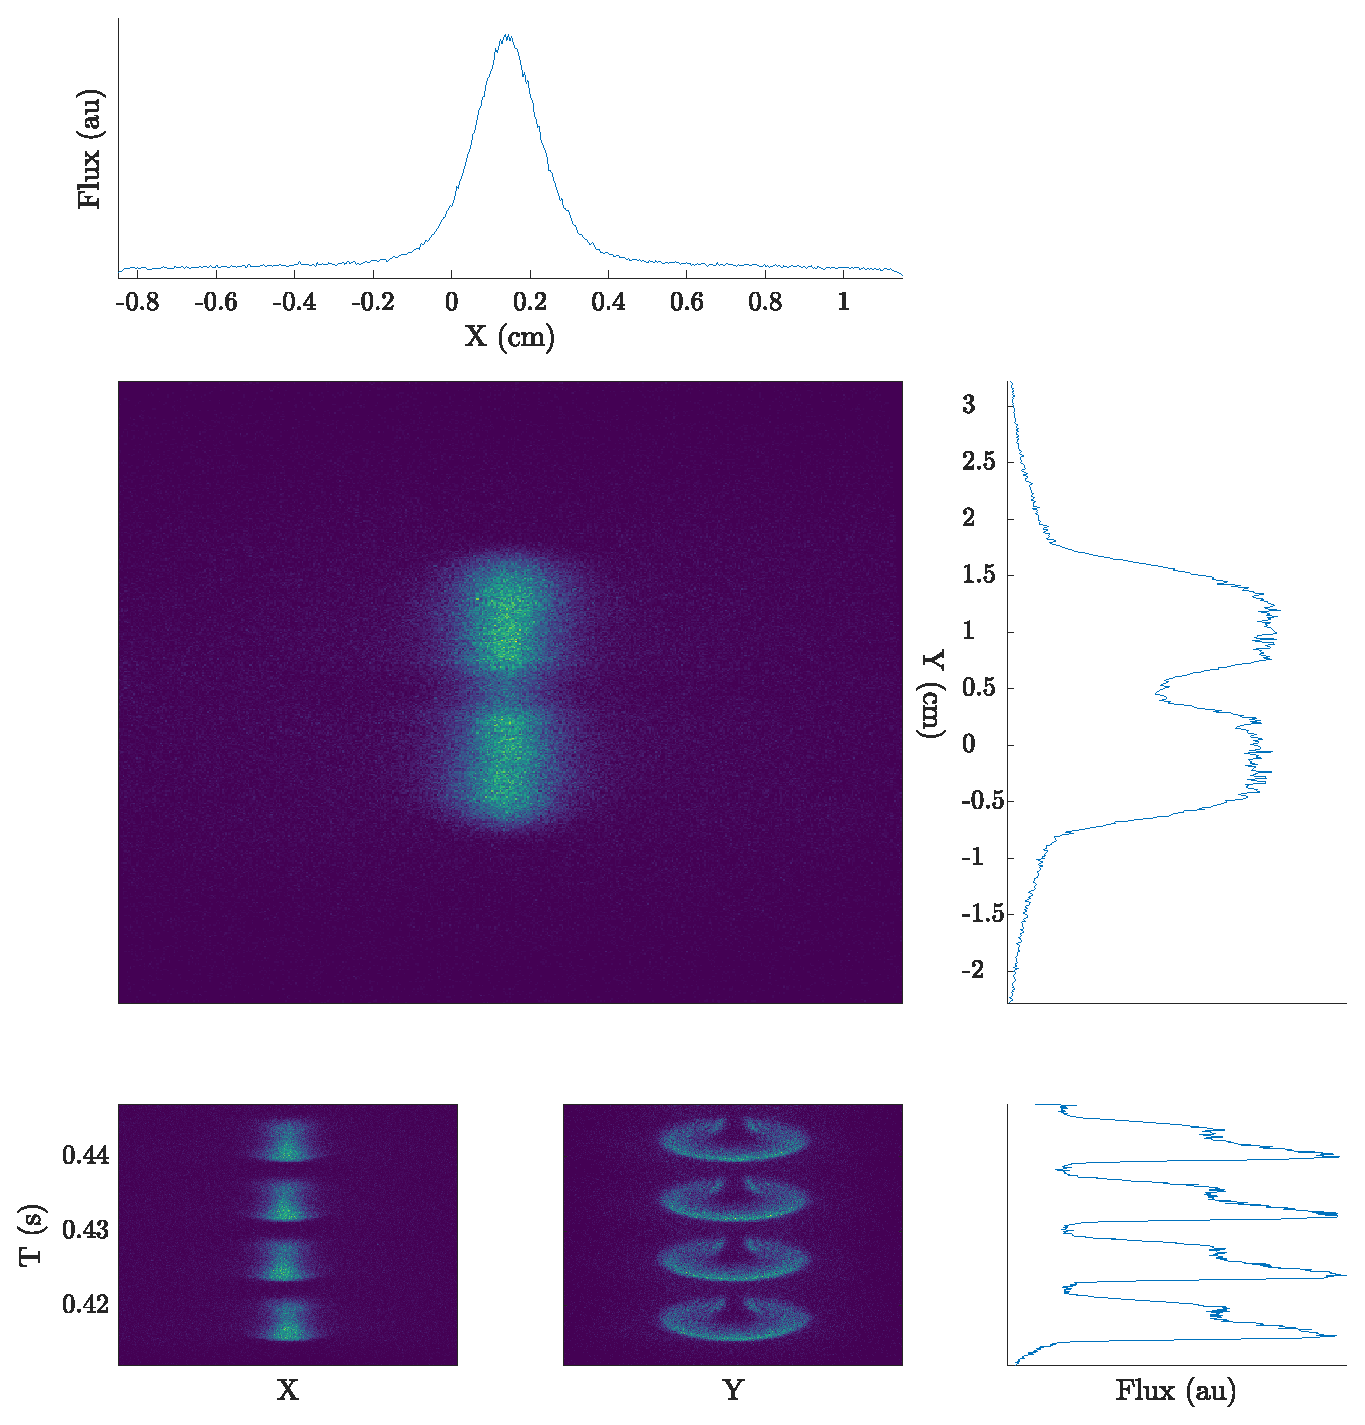
\includegraphics[width=\textwidth]{fig/apparatus/pal_MCP_micro}
	 	\caption{MCP readout of the first few pulses from a pulsed atom laser.}
	 	\label{fig:pal_micro}
	 \end{figure}
	 \todo{Without the reader knowing about atom lasers, they may think that these images look even more saturated than teh BEC!  The spatial profile certainly looks much worse.  You should at least mention that mean-field effects cause several types of distortion, and cite our earlier papers.}
	 \newpage

% PAL picture is integrated over 156 shots from 5_3d_2_3 data
% QD picture is integrated over about 1300? in tight trap fwiw from run 8

% PAL parameters; 1.6-3 MHz centering (see that ol plot) depending on trap
% pulsees 6-12 cycles
% typically sampled at 6-11 ms periods, generally limited by BEC width
% 


% tcpip interface for laser lock
% 	t = tcpip(IP, 33333, 'networkrole','server')
% 	fopen(t)
% 	fwrite(t,freq,'double')
% 	fclose(t)

% And on the other end - a loop that hammers it with queries?
% init parallel pool
% 	if workerID == 1
% 		while true
% 			try
% 				t = tcpip('localhost',33333,'networkrole','client')
% 				fopen(t)
% 				setpt = fread(t,1,'double')
% 				fclose(t)
% 				labSend(setpt,2)
% 			end
% 		end
% 	elseif workerID ==2 
% 		solstis = find_instrument();
% 		instrument_status = getResponse(solstis)

% 		write_logfile(instrment_status,metadata)
% 		% Omitting parameters for lock loop like wait times, slew rate limits, etc, various timers,

% 		if labProbe
% 			data = labReceive(1);
% 			if data != setpoint
% 				old_setpoint = setpoint;
% 				setpoint = data;
% 		red_freq = WM_query();
% 		PID_step(red_freq,setpoint,parameters)


% -> Something about communication between parallel workers?
% Ethernet link between PC and solstis driver; query returns machine state like internal photodiode readings and optomechanical actuator voltages


\section{Vacuum system integration}
	
	% Physical models often make simplifying assumptions, like ignoring air	resistance or friction, or collisions etc. Idealized models are only	solvable in certain special cases, and introducing nonlinear effects	like friction can make them mathematically intractable. This is	partially resolved by sophisticated modelling these days, but the	approximations will always remain. So when it came to studying	microscopic systems, one would like to remove the background. so that	the thing you are examining becomes not only the foreground, but the	only thing in the image, and so your signal is not obfuscated. So people	have tried to make vacuum for quite some time! Indeed this is one way	atmospheric pressure was measured - 

	While nature abhors a vacuum, experimentalists abhor a background. Ultracold atom experiments require ultra-high vacuum (UHV) conditions because collisions with a background gas can easily overcome the frail forces that hold the atoms in their traps. Our vacuum is maintained by continuous operation of several turbomolecular pumps\footnote{One of the earliest accomplishments of significant vacuum was by Lavoisier, who used pumps from the firestation to evacuate a chamber. Since then vacuum has advanced considerably, and at ultrahigh vacuum the exhaust is so dilute that one does not have the viscosity to operate pumps in the true sense. Nonetheless, the name remains.}, which are backed by roughing pumps. For the UHV chambers where BEC is created, an additional turbomolecular pump operates between the vacuum-adjacent turbo and the roughing pump.  Contamination of the vacuum chamber interior occurs from environmental sources like atmospheric pollutants or errors while handling components. When first pumping down to vacuum, contamination by water, oils, dust, or other materials can prevent achievement of good vacuum because of outgassing of volatile chemicals within the contaminant. These surface contaminants can be removed by wrapping the machine in heater tapes and insulating aluminium foil, and baking at up to 150 degrees celsius for several days. In this process one typically observes a sharp rise in pressure as the chamber heats and the contaminants volatilize, and then a decrease to a lower steady-state pressure as the contaminants cease outgassing and the remnants are evacuated. Once the pressure stabilizes, the heater tapes can be turned off, and as the apparatus cools the pressure will settle to a more preferable level. 
	% Care must be taken not to heat or cool the machine too quickly, or differences in thermal expansion between connected flanges can open leaks to atmosphere and undo much patient work. 

	% In the course of my scholarship, I extended the vacuum system of the lattice machine by constructing the LVIS, science chamber, and detector chambers. 

	Even after baking, the pressure may not be low enough to permit long-lived traps. Hydrogen leaching from the surface of the steel chamber can be significant. One method of dealing with this is by titanium sublimation. Specialized `titanium sublimation pumps' pass a large current (several amps, pulsed) through a titanium filament which sublimates titanium atoms that eventually adsorbs on the walls of the chamber. Hydrogen adsorbs to the titanium surface but not to steel, and so after some applications the pressure trends further down. Further reduction in hydrogen background can be achieved by so-called `getters', which present a highly porous surface into the vacuum and to which Hydrogen is strongly adsorbed. The chemical makeup of the background pressure can be determined using residual gas analysers (RGAs) which are essentially compact mass spectrometers. They can help diagnose whether one has an air leak or organic contaminant, and are helpful for leak hunting when paired with a bottle of helium gas, gently vented near suspect flanges.
	\todo{This paragraph is typical of a lot of this chapter - a general introduction and vague description, but no specifics as to what we actually do!  E.g. from this I'd assume we have Ti subs on both machines.  Remember that your thesis is meant to talk about what you did, and this chapter in particular should describe the machines you worked on much more than provide a general introduction to the experimental aspects of BEC machines.}

	The vacuum systems form the skeleton of both machines, which have a common structure illustrated schematically in \ref{fig:vacuum_diagram}. The placement of some of the turbomolecular pumps, faraday cups, and pressure gauges differ between the machines, but this makes no functional difference. However, the beamline of the lattice machine does not feature a deflection stage or a focus for the LVIS. Otherwise, the overall structure of the vacuum systems is the same and so only the BiQUIC machine is shown in its entirety in in Figure \ref{fig:vacuum_diagram}. \todo{put figures closer to references}

	\begin{sidewaysfigure}
		\centering
		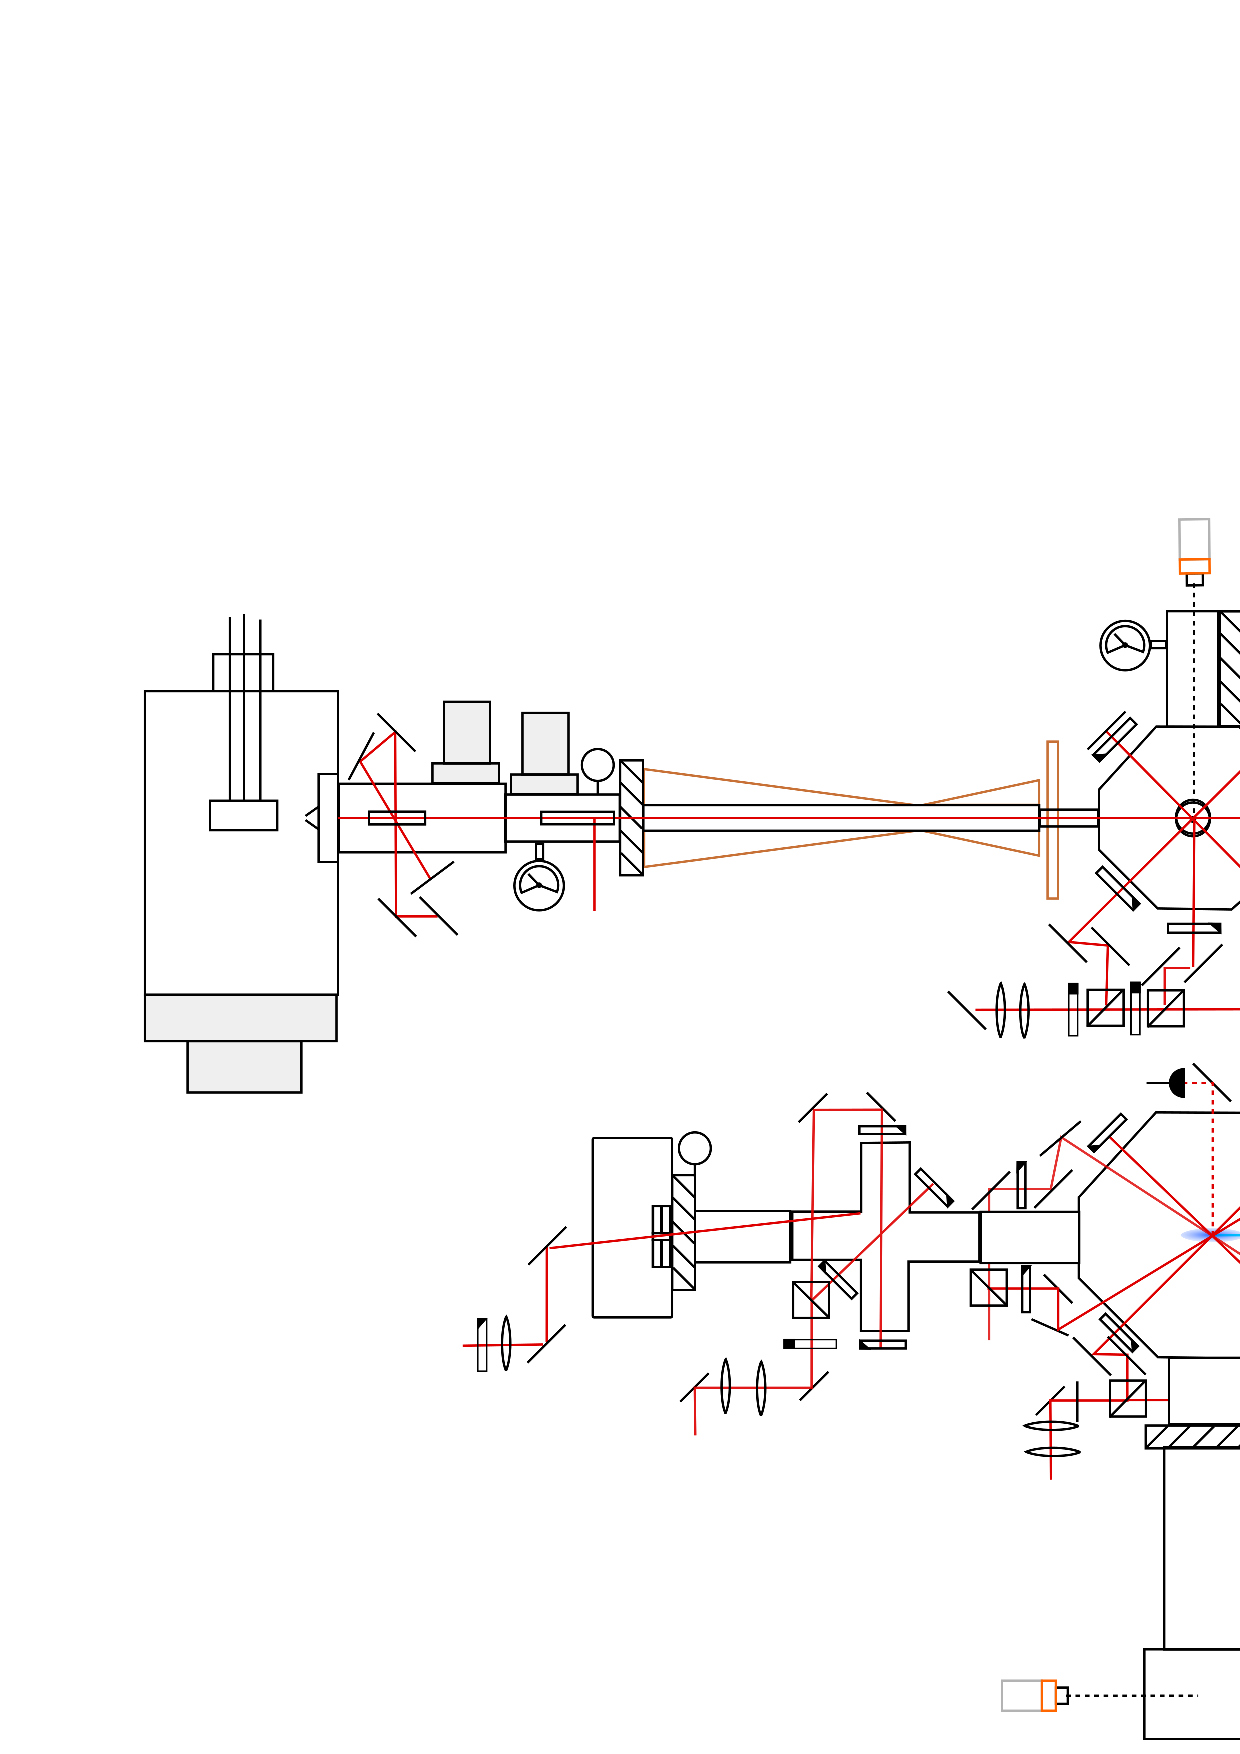
\includegraphics[width=\textwidth]{fig/apparatus/vacuum_schematic}
		\caption{Vacuum system and laser insertion optics used in the downstairs experiment \todo{These diagrams are pretty confusing... At least you need to add some labels to parts of the vacuum system, different beams etc.  A legend showing different components might help too.  In general, a diagram such as this trying to show every optical component isn't very helpful - the reader doesn't need to know about every lens and mirror in every beam path!}}
		\label{fig:vacuum_diagram}
	\end{sidewaysfigure}
	


	A major difference between the two setups is the construction of the chamber housing the final trapping stage in which BEC is achieved. the BiQUIC machine has more limited optical access and has featured the spectroscopic laser, as depicted in Figure \ref{fig:vacuum_diagram}. For comparison, the apparatus around the lattice machine's science chamber is shown and described in Chapter \ref{chap:lattice}. \todo{Probably just make this chapter exclusively about the BiQUIC machine. Differentiate the machines in the lattice chapter.}
	% This machine features 8" re-entrant windows on each face of a large Kimball chamber as well as several 3.25" (?) windows for insertion of the dipole and (eventually) lattice beams. In commparison, the science chamber of the BiQUIC machine has been running with coils built in the BiQUIC configuration for many years, but the coil housing itself precludes large windows.
	% The horizontal MOT beams in this case are limited to about 1cm diameter. The diagonal beams, in-trap cooling beams, and Bragg beams (when they are used) are inserted through small windows (1"?) protruding from the sides of the chamber.


	 %- what fraction would have sufficiently low	energy to capture, and how long would they last? 
	


\section{Data acquisition \& control}

	Control of the optical components (AOMs and shutters), coil current supplies, and RF radiation is coordinated by a central LabView program which transmits pulse sequences to the machine via National Instruments pulse cards. The cards themselves are connected to the CPU by a PCI bus, and synchronize their internal clocks at the beginning of each shot. The cards also record analog inputs such as Fabry-Perot cavity scan traces, photodiode traces, and mains voltage traces for post-processing diagnostics.

	The LabView software is old, and the absence of documentation made significant modifications impractical. A workaround was accomplished by including a command that calls a specified MATLAB subroutine (referred to as the `interface'), which is customizable to suit the purposes of a given experiment\footnote{The software developed to analyse the data from various experiments is invariably written in MATLAB. Many core capabilities are stored in the repository \url{https://github.com/HeBECANU/Core_BEC_Analysis}, and generally each project will have a unique public repository as well.	}. This subroutine can pass a \verb|.xml| file path to a LabView pulse sequence file to use in the next experimental cycle, and even modify the sequences, albeit in a limited way due to the particulars of LabView's sequence specification format. This extension allows for automatic optimization of experimental sequences, as was demonstrated in \cite{HensonML}, but obviously is of no use for mechanical tasks like beam alignment\footnote{One can dream, though.}. 
	\todo{Remove above para and fix flow}
	The interface script also writes metadata to a log file, including the POSIX timestamp, type of shot executed (e.g. \verb|calibration| or \verb|AtomLaser|), shot number, and other relevant parameters. The timestamps in this logfile can be cross-referenced with the \verb|*d.txt| files that are written by the TDC computer and with the LabView logs of analog inputs in order to match the experimental parameters with data files for post-processing purposes. The data analysis pipelines for modern experiments can be complex, and the experiments in this thesis generally comprise a handful of different diagnostics processed in parallel. The tagging of shots by timestamp cross-referencing allows separation of relevant shots for each processing subroutine. 
	An example of the detailed diagnostics produced from the logs and metadata are shown in Figure X \todo{diagnostic figure}

\subsection*{Optimizing machine performance}

	% Routine maintenance is required to keep the machine capable of producing large condensates. Despite the stabilized environment, optics are prone to wander slightly over time. The stable temperature is especially important as the cooling beams are coupled from the AOM tables to the vacuum chamber optics by free-space links. Drift in the relative position of the optics tables would therefore result in misalignment of many laser beams, and degrade performance of the machine. The conditioned air is supplied through three HEPA filters in the lab ceiling. The resulting positive pressure in an area enclosed by PVC strip walls keeps dust from entering the area on air currents. 

	If the second MOT is loading and a saturated fluorescence signal is visible, one can usually optimize all of the optical alignments on this signal, which is a factor of ten faster than the full BEC creation sequence. If this is not available, historical records of diagnostics taken at several points throughout the beamline can facilitate diagnosis of the point of failure. The most commonly employed tests are faraday cups which produce a current when impacted by \mhe atoms, as read out on a picoammeter. These current sensors are placed after the deflection stage, at the end of the Zeeman slower (with a large hole bored through it to allow the slowing beam to pass through), between the first MOT and the focus stage, and behind the second MOT chamber. In case the first MOT is not operational, a Xenics Bobcat CCD camera mounted above the chamber provides a view of the trapping region and direct visual feedback about the presence, shape, and density of the MOT. 


	% A more elegant solution could take the form of a main script that generates control pulses, absorbs the functions of the interface while monitoring the TDC output directory, and creates a direct link between log files and the \verb|d.txt| files. Unfortunately, even if LabView were able to provide all this functionality, upgrading the control software would be like moving deckchairs on the titanic. It would be more effective to replace the entire control suite, which could take several months. Given the long build times required for new experiments, during which continuous operability is essential, and that adjusting the control software is a relatively small part of the demands of operator time, this upgrade is not a high priority.  However, the control software for Staggering Grace was recently upgraded to a more readily usable and modifiable Python-based infrastructure, which will surely prove both helpful and informative for future designs.

    % \begin{figure}
    % 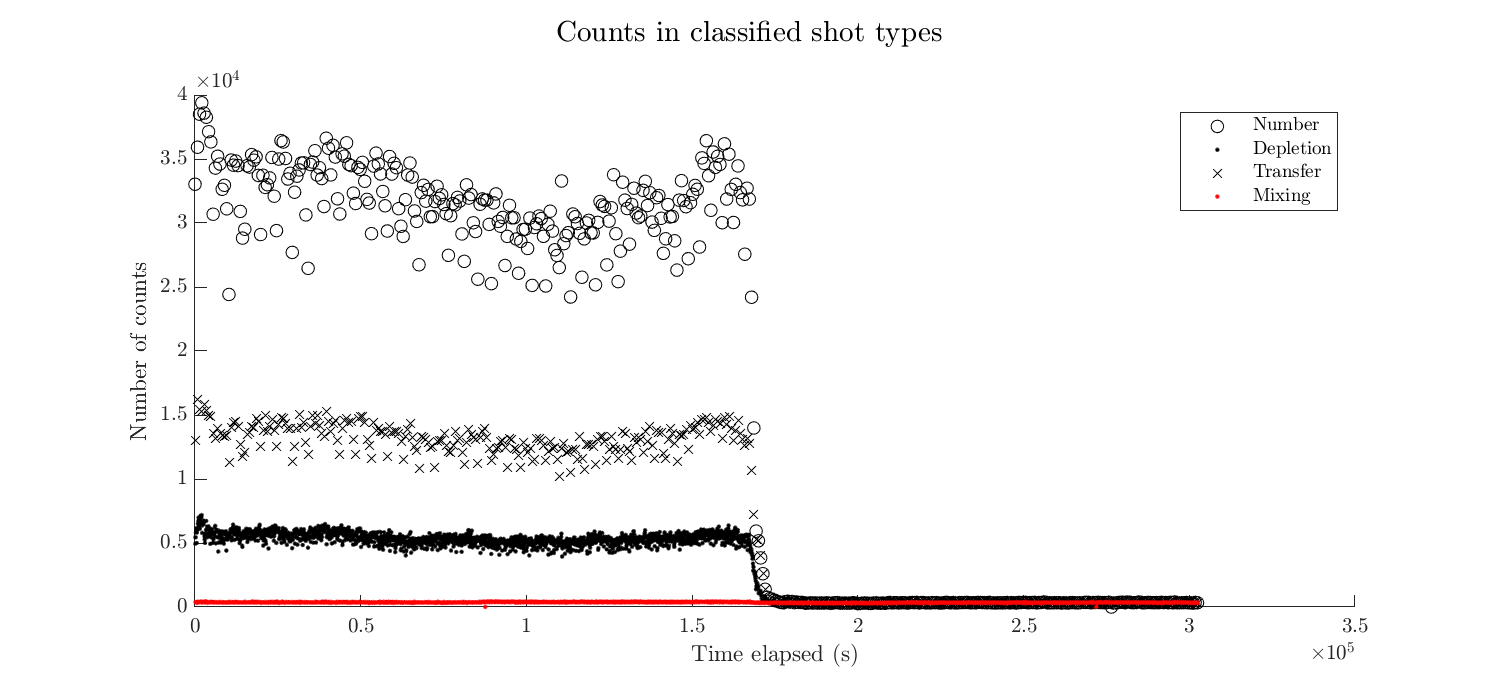
\includegraphics[width=\textwidth]{fig/depletion/partition_QD_files_01_shot_counts_combine}
    % \label{fig:qd-count_by_type}
    % \caption
    % \title
    % \end{figure}





   
 %   Notes on new BEC paper
	% We report the realisation of Bose-Einstein condensation (BEC) of metastable helium atoms using an in-vacuum coil magnetic trap and an optical dipole trap. A novel quadrupole-Ioffe configuration (QUIC) magnetic trap made from in-vacuum hollow copper tubes provides fast switching times while generating traps with a 10G bias without compromising optical access. The bias enables in-trap 1D doppler cooling to be used, which is the only cooling stage between the magneto-optic trap (MOT) and the optical dipole trap. This allows direct transfer to the dipole trap without the need for any additional evaporative cooling in the magnetic trap. The entire experimental sequence takes 3.5 seconds, with essentially pure BECs observed with ∼ 1e6 atoms after evaporative cooling in the crossed dipole trap.

	% Get Herwig Ott paper [7] for thesis ref

	% Collim 67Isat, -5Gamma
	% 5W fibre amp for cooling beam
	% ZS 92Isat -160Gamma
	% MOT1 87Isat horz 110ISat vert -22Gamma detuning
	% 1.5mm hole in chamber
	% <3e-11 mTorr
	% push 110Isat 3.5Gamma for low-velocity intense source LVIS
	% Flux into 2nd MOT is 9e8 atoms/sec using faraday cup and picoammeter
	% Second MOT gradient 4.4G/cm (in weak or strong axes?)
	% -33Gamma and 140, 37 Isat
	% 1.7e8 atoms loaded at 2.5mK in 1 second, as measured using saturated fluro on an InGaAs PD [26]
	% 451mm fall to detector
	% 	DLD not operational yet so measure the current pulses on the plates frmo the charge depletion when atoms impact the plates. Fast amplifier and a discriminator then recorded using a digital counter to extract 1D tof distribution.
	% MOT compression - ramps to 1.42G/cm in 10ms while linearly ramping lasers to -0.4Gamma and decreasing intensity by a hundredfold, then switching off and the +1s remain trapped
	% Then compress the mag trap to 16.6G/cm in 100\mu s, and ramp the bias up in 100ms to provide a 10G bias in the QUIC trap. Has radial 89Hz and 57Hz z freqs. Have 5.3e7 atoms at 0.44mK. Measured using absorption imaging along the x axis using an InGaAs CCd. Flipper mirrors allow operation on the MOT axis but mean imaging not available during MOT.
	% 1D Doppler cooling [tychkov paper 25], with .01Isat and sigma+ polz directed vertically down along the bias direction. Detuned -Gamma/2.  After 500mss have 4.9e7 atoms at 83\mu K. Ready for dipole transfer.
	% 100kHz seed at 1550nm feeds a 30W amplifier, but produces 6W (y axis) and 1W (10degrees from X, in the XY plane) after AOM and fibre coupling losses. Waists are 73 and 55 micron respectively, crossing the centre of the biased trap, 6mm above the centre of the horz coils
	% Trap freqs 1.1,1.2,1.7 kHz and 150muK deep
	% Doppler cooling seems more effective with dipole beams on as it works at better at high density [25 tychkov] - indeed improving final atom number by some 50%. So they are ramped on over 100ms prior to doppler cooling
	% QUIC trap linearly relazed to an unbiased trap with 1.1G/cm gradient and then switched off with a FET. Additional square coil is switched on to create a uniform 1.6G field pointing in z direction. Turned on before the QUIC rampdown starts. Eventually found that the earth's field was sufficient to maintain the quantiation axis and suppress Penning ionization, so is switched off after 700ms in ODT. Measure 5e6 atoms at 13.5muK, 0.5 PSD
	% Trap depth reduced by exponential rampdown of power over 1 sec. 

	% Can extract mu via R_tf ^2 / 2t_tof ^2, and so from TF picture get N_0 = (2mu)^{5/2}/(15\sqrt{m}\hbar\bar{\omega}^3 a).
	% Cross T*_c at 6\mu K with 3e6 atoms, down to 80% BEC with 1e6 atoms


	% is that supposed to be a dot product?. The dipole potential is proportional to the intensity and the real part of the polz, which descrives the in-phase component of hte oscillation. The force is given by the gradient of this potential. The absorption from the driving field (and reimission in steady-state) is 
	% $P_{abs} = \langle\dot{\textbf{p}}\textbf{E}\rangle = \frac{\omega}{\varepsilon_0 c}Im(\alpha) I$. The scattering rate is therefore $P/\hbar\omega$. The Lorentz oscillator considers an electron with an SHO-like elastic binding to a fixed nucleus, with natural freq $\omega_0$ and a damping rate $\Gamma$. The resulting DE 
	% $x''+\Gamma_{\omega}x'+\omega_0^2x = -e E(t)/m_e$ includes the natural decay rate 
	% $\Gamma_{\omega} = e^2\omega^2/6\pi\varepsilon_0 m_e c^3$, which gives a solution for 
	% $\alpha=\frac{e^2}{m_e}\frac{1}{\omega_0^2-\omega^2-i\omega\Gamma_\omega}$. 

	% In the limit of large detunings, negligible saturation, and in the rotating wave approx, one finds
	% $$
	% U_{dip}(r) = \frac{3\pi c^2}{2\omega_0^3}\frac{\Gamma}{\Delta}I(r),
	% $$
	% $$
	% \Gamma_{sc} = \frac{3\pi c^2}{2\hbar\omega_0^3}\left(\frac{\Gamma}{\Delta}\right)^2I(r),
	% $$
	% Yielding the useful relation $\hbar\Gamma_{sc} = \Gamma U_{dip}/\Delta$, indicating two important principles: The scaling with intensity and detuning, and the importance of the sign of the detuning.

	% In multilevel atoms, one can extend the argument to other higher-lying states and compute the polarizability farther from several resonances, which leads towards tuneout wavelenghts...


	% This semiclassical model captures the absorption and stimulated emission of light from an electromagnetic field, but does not explain spontaneous emission. A fully quantum-mechanical treatment of the system (such as the Jayne-Cummings model) will also fail in this respect. The mechanism of spontaneous emission requires the theory of QED for a full explanation, wherein vacuum fluctuations produce short-lived virtual particles - including photons - which occasionally have the right wavelength to stimulate emission from atoms. We will not explore this detail here, but remain satisfied with the natural lifetime 
	
	


	% The interaction of an electric field with an atom induces a dipole $-e\textbf{r} - \varepsilon_0 \chi_a \textbf{E}$, where $\varepsilon_0\chi_a$ is the scalar polarizability (there are higher terms, as treated later). The interaction energy is 
	% $U=-\frac{1}{2}\varepsilon_0\chi_aE^2$ - by reference to the work above. The force follows from $F = -\nabla U$. A radiation field with frequency $z$ propagating along the $z$ direction gives rise to a force, averaged over timescales much larger than $1/\omega$, which can be written in terms of the Bloch components
	% $$
	% \bar{F}_z = \frac{-\hbar\Omega}{2 E_0}(u\frac{\partial E_0}{\partial z} - v k) = F_{dipole}+F){scatt},
	% $$

	% where $k$ is the wavenumber of the light, finally giving rise to 
	% $$
	% F_{scatt} = \hbar k\frac{\Gamma}{2}\frac{\Omega^2/2}{\delta^2+\Omega^2/2+\Gamma^2/4}
	% $$

	% $$
	% F_{dipole} = -\frac{\hbar\delta}{2}\frac{\Omega^2}{\delta^2+\Omega^2/2+\Gamma^2/4}\frac{\partial\Omega}{\partial z},
	% $$
	% The latter goes to zero on resonance ($\delta=0$). This argument applies for all three spatial dimensions and so one arrives at $U_{dipole} \approx \frac{\hbar^2\Omega}{4\delta}$, once again. One can also arrive at a similar expression for the radiative force by considering a simple model of photons with wavenumber $k$ being absorbed and emitted at a rate $\Gamma$, where the re-emission process imparts a zero impulse on average, but is limited in temperature.
	% from \cite{Grimm00}


	% An experimentalist is occasionally required to negotiate the geometry of trapping fields, laser beams, and polarization vectors in order to correctly configure optics. A method follows.

	% For an electric field propagating with a wavevector $\vec{k}$ in the lab frame across an atom in a magnetic field $\vec{B}=B\hat{\vec{B}}$...
	% 	The electric field of a purely polarized light ray at a point in space can be expressed as

	% $$
	% \textbf{E}(t)=\begin{bmatrix}
	% E_x(t)\\
	% E_y(t)\\
	% E_z(t)
	% \end{bmatrix}
	% $$

	% If we fix the axis of propagation to be $\hat{z}$, then we can write

	% $$
	% \textbf{E}(t)=\begin{bmatrix}
	% E_{x0} e^{i(kz-\omega t -\phi_x)}\\
	% E_{y0} e^{i(kz-\omega t -\phi_y)}\\
	% 0
	% \end{bmatrix}
	% $$

	% We can then define the Jones vector $\textbf{J}_0 = \left(E_{x0}e^{i\phi_x},E_{y0}e^{i\phi_y}\right)^T$, so $\textbf{E}(t) = \textbf{J}e^{i(kz-\omega t)}$.

	% In this frame, the amplitudes of horizontal and  vertical polarization are $E_{x0}$ and $E_{y0}$ respectively. Therefore, diagonal polarization is a linear combination of both these components, and circularly polarized light is a linear combination with an imaginary coefficient. 
	% A shortcoming of the Jones calculus is that it is only applicable to light which is completely polarized (that is, for some basis it can be written as $\textbf{E} = (E_0,0)$). This is not true for a beam whose polarization varies, or where there are power fluctuations in one of the axes, etc. There should be a single motivating example somewhere, but these are some examples. If this assumption is not permitted - by which measurement would you tell the difference? - then we must move to the Mueller calculus. %Determining purity of polz empirically


	% When working with two-level systems it is convenient to introduce the density matrix $\rho$. The assumption that the system must always be in \emph{some} state can be written as the normalization condition
	% \begin{align}
	% 	1&=\sum_i |\braket{\phi_i}{\psi}|^2\\
	% 	 &= \sum_i \braket{\phi_i}{\psi}\braket{\psi}{\phi_1}\\
	% 	 &= \textrm{Tr} \rho,
	% \end{align}
	% where the Trace operation is defined by $\textrm{Tr}(\ket{a}\bra{b})=\braket{b}{a}$. 
	% The density matrix permits a statistical approach to ensembles of conditional states, which will be useful in later chapters, and unifies the treatment of the important features of atom-light interactions, which is the subjects of the rest of this section. \footnote{The density matrix formalism also allows for treatment of statistical mixtures of quantum states on equal footing with so-called `pure' states which are certain to be in some state $\ket{\psi}$. While the normalization condition is guaranteed to hold for any $\rho = \sum_i p_i\hat{rho}_i$, there is no such way to write mixtures in the form $\ket{\Psi}=\sum_i\ket{\psi_i}$ without violating the assumption of conservation of probability. Indeed, pure states, defined by $\textrm{Tr}(\rho^2)=1$, are quite exceptional: They are a set of zero measure in the set of all positive semidefinite Hermitian operators with unit trace.}. When expressing the state  in terms of the energy eigenbasis $\{\ket{n}\}$, the diagonal elements $\rho_{ii}\in\mathbb{R}$ are the \emph{populations} of the $i^{\text{th}}$ eigenstate and the off-diagonal \emph{coherences} $\rho_{ij}=\rho_{ij}^{*}$ capture the utility of the quantum state for interferometric purposes\footnote{In what sense? c.f. Ramsey interferometry}. 

	% By working in a rotating reference frame via the change of basis\footnote{This change of basis induces a change to the coefficients $c_n=\exp((-1)^n \delta t/2)$} $\hat{U} = \textrm{diag}(e^{i\delta t/2},e^{-i\delta t/2})$, in terms of the detuning $\delta=\omega-\omega_0$, one can write the Hamiltonian in the convenient form \cite{FootAtomic}

	% \begin{equation}
	% 	\hat{H} = \frac{\hbar}{2}\begin{pmatrix}\delta&\Omega\\
	% 											\Omega&-\delta\end{pmatrix},
	% \end{equation}
	% which has eigenvalues $E'_\pm = \pm \sqrt{\delta^2+\Omega^2}/2$, retaining the bare splitting $\delta$ between levels when $\Omega=0$. In the presence of an oscillating field which drives an allowed transition, i.e. when $\Omega>0$, the energy of the \emph{dressed state} of the atom are shifted with respect to their unperturbed values

	% %  For now we will simply note that the average of a set of measurements of the quantity $Q$ on an identically-prepared system can be calculated via the expectation value of the corresponding operator $\hat{Q}$,
	% % \begin{align}
	% % 	\langle Q\rangle &=  \bra{\psi} \hat{Q}\ket{\psi}\\
	% % 	&= \textrm{Tr}(\hat{Q}\rho),
	% % \end{align}
	% % and that the time-dependence of the expected value follows from Ehrenfest's theorem
	% % \begin{equation}
	% % 	i\hbar \frac{\partial}{\partial t}\langle Q\rangle = [\hat{H},\hat{Q}],
	% % \end{equation}
	% % which holds equally well for the density matrix, providing the von Neumann equation $\dot{\rho} = i[\rho,\hat{H}]/\hbar$.
	
	% Let us concern ourselves with a further simplified picture of the atom as well: Indeed, we model the atom with the simplest nontrivial quantum system, one with only two distinguishable states. A two-level system permits convenient expression of the entire density matrix
	% \begin{equation}
	% 	\hat{rho} = \begin{pmatrix}
	% 		\rho_{11}&\rho_{12}\\
	% 		\rho_{21}&\rho_{22},
	% 	\end{pmatrix}
	% \end{equation}




	% The wavefunction $\Psi$ of an electron of mass $m_e$ moving in a central potential $V(r)$ can be written in terms of the bound eigenfunctions (also called \emph{orbitals}) of the Schr\"{o}dinger equation
	% \begin{equation}
	% 	\left(\frac{-\hbar^2}{2m_e}\nabla^2 + V(r)\right)\psi_{nlm} = E_n\psi_{nlm},
	% \end{equation}

	% which have the form


	% On the optical Bloch equations;
	% Starting from the density matrix, 
	% $$
	% \begin{bmatrix}
	% \rho_{11} & \rho_{12}\\
	% \rho_{21} & \rho_{22}
	% \end{bmatrix} = \ket{\Psi}\bra{\Psi},
	% $$
	% We make the unitary transformation into a rotating frame by $U=\exp(diag(-i\delta t/2,i\delta t/2))$, which is a gauge transformation such that the zero energy is exactly between the upper and lower states, 
	% $\delta=\omega-\-\omega_0$. This looks like a transformation $U = \exp(-i\sigma_z t)$ where $\sigma_z$ is the first of the Pauli matrices which generate the unitary group of dimension 2. In the rotating frame one then has the Bloch vector defined by 
	% $R_i = Tr(\rho\sigma_i)$. One can then transform the differential equations for $c_i$ into the rotating basis and obtain the time evolution of the system which can be conveniently written in the form $\dot{R} = R\times W$ where $R$ is the Bloch vector and $W=\Omega\hat{e}_1+\delta\hat{e}_3$.  
	% One can include damping by adding a decay term of the form $\dot{\rho}_{22} =-\Gamma\rho_{22} + \Omega \sigma_y/2$, which recovers the exponential decay of the excited state in the absence of a driving field. We finally have the optical bloch equations, which (may) still be expressible in a neat vector form?
	% $$
	% \dot{u} = \delta v - \Gamma u/2\\
	% \dot{v} = -\delta u + \Omega w - \Gamma v/2\\
	% \dot{w} = -\Omega v - \Gamma(w-1)
	% $$, 
	% which capture the population dynamics of a two-level atom coupled to a radiation field near resonance with significant spontaneous decay. A similar procedure can be extended to many-level atoms (one-two-many quote), and is employed in chapter X appendix Y to predict the SNR of interrogating the forbidden transition.

	% In the rotating frame one can write the Schrodinger equation in terms of the amplitudes in the rotating frame 
	% $$
	% i\frac{d}{dt}(\tilde{c}_1,\tilde{c}_2) = \begin{bmatrix}\delta/2&\Omega/s\\\Omega/2&-\delta/2\end{bmatrix}(\tilde{c}_1,\tilde{c}_2),
	% $$

	% which has eigenvales $\lambda = \pm(\delta^2+\omega^2)^{1/2}/2$ - which reproduces the raw splitting $\delta$ in the absence of a field. When $\Omega>0$ - see Cohen-Tannoudji for a deeper treatment of this dressed state picture. When the detuning is much larger than the rabi frequency then one gets $\lambda\approx\pm(\delta/2 + \Omega^2/4\delta)$, which is the bare detuning with a light shift given by the second term. The sign of the shift is given by the detuning. This light shift, or AC stark shift, is what underpins the working of the dipole force. 
	% Dipole beams are widely used in biophysical contexts for manipulation of DNA, proteins, and even entire bacteria. See Ashkin 1997 or Lang and Bloch 2003?
	% $\varepsilon$
	
	% Radiation pressure traps afew K deep, can cool to some 10s of $\mu$ K
	% Typical dipole traps less than a mK deep!
	


	% RGL Theory of AC stark shift for polz; [107-108] theory, latter Lorentz oscillator model, treats as SHO basically? Which is damped by emission of radiation - gives  second order ODE which can be solved. Good for weak driving. 
	% Of course, corrections are needed when other transitions are important, i.e. when fairly close to a strong line
	% RGL [109] second order perturbation sums over all possible final states. 
	% % Sobel'man I, introduction to the theory of atomic spectral Pergamon press 1972
	% show that the polzability can be written in the familiar alpha eqn 
	% % A Derevianko, H katori, physics of optical lattice clocks, rev mod phys 83, 2011
	% % J R P Angel, P G H sandars, the hyperfine structure STark effect, proc roy. soc. a, 305 1968		